\section{Разработка парсера}

\subsection{Задание}
Арифметические выражения в постфиксной записи.

\subsection{Построение грамматики}
Построим грамматику.

\begin{tabular}{ r c l }
    $E$ & $\to$ & $EEO$ \\
    $E$ & $\to$ & $n$ \\
    $O$ & $\to$ & $ + | * | - $ \\
\end{tabular}

\begin{center}
    \begin{tabular}{ | l | l | }
        \hline
        \textbf{Нетерминал} & \textbf{Описание} \\
        \hline
        $E$ & Начальный нетерминал, выражение \\
        \hline
        $O$ & Операция. \\
        \hline
    \end{tabular}
\end{center}

Избавимся от левой рекурсии.

\begin{tabular}{ r c l }
    $E$ & $\to$ & $nC$ \\
    $E$ & $\to$ & $n$ \\
    $C$ & $\to$ & $EOC$ \\
    $C$ & $\to$ & $EO$ \\
    $O$ & $\to$ & $ + | * | - $ \\
\end{tabular}

\begin{center}
    \begin{tabular}{ | l | l | }
        \hline
        \textbf{Нетерминал} & \textbf{Описание} \\
        \hline
        $E$ & Начальный нетерминал, выражение \\
        \hline
        $O$ & Операция. \\
        \hline
        $C$ & Продолжение выражения, левая рекурсия \\
        \hline
    \end{tabular}
\end{center}

Избавимся от правого ветвления.

\begin{tabular}{ l c l }
    $E$ & $\to$ & $nE'$ \\
    $E'$ & $\to$ & $C$ \\
    $E'$ & $\to$ & $\varepsilon$ \\
    $C$ & $\to$ & $EOC'$ \\
    $C'$ & $\to$ & $\varepsilon$ \\
    $C'$ & $\to$ & $C$ \\
    $O$ & $\to$ & $ + | * | - $ \\
\end{tabular}

\begin{center}
    \begin{tabular}{ | l | l | }
        \hline
        \textbf{Нетерминал} & \textbf{Описание} \\
        \hline
        $E$ & Начальный нетерминал, выражение \\
        \hline
        $E'$ & Продолжение выражения, правое ветвление \\
        \hline
        $O$ & Операция. \\
        \hline
        $C$ & Продолжение выражения, левая рекурсия \\
        \hline
        $C'$ & Продолжение выражения, правое ветвление \\
        \hline
    \end{tabular}
\end{center}

Построим множества \textbf{FIRST} и \textbf{FOLLOW} для нетерминалов.

\begin{tabular}{| l | l | l |}
    \hline
    \textbf{Нетерминал} & \textbf{FIRST} & \textbf{FOLLOW} \\
    \hline
    $E$ & $n$ & \$, $+$, $*$, $-$ \\
    \hline
    $E'$ & $n$, $\varepsilon$ & \$, $+$, $*$, $-$ \\
    \hline
    $C$ & $n$ & \$, $+$, $*$, $-$ \\
    \hline
    $C'$ & $\varepsilon$, $n$ & \$, $+$, $*$, $-$ \\
    \hline
    $O$ & $+$, $*$, $-$ & $n$, \$, $+$, $*$, $-$ \\
    \hline
\end{tabular}

\section{Тестирование и визуализация}
\subsection{Тест 1}

\texttt{1 2 10 + *} --- тест из условия.

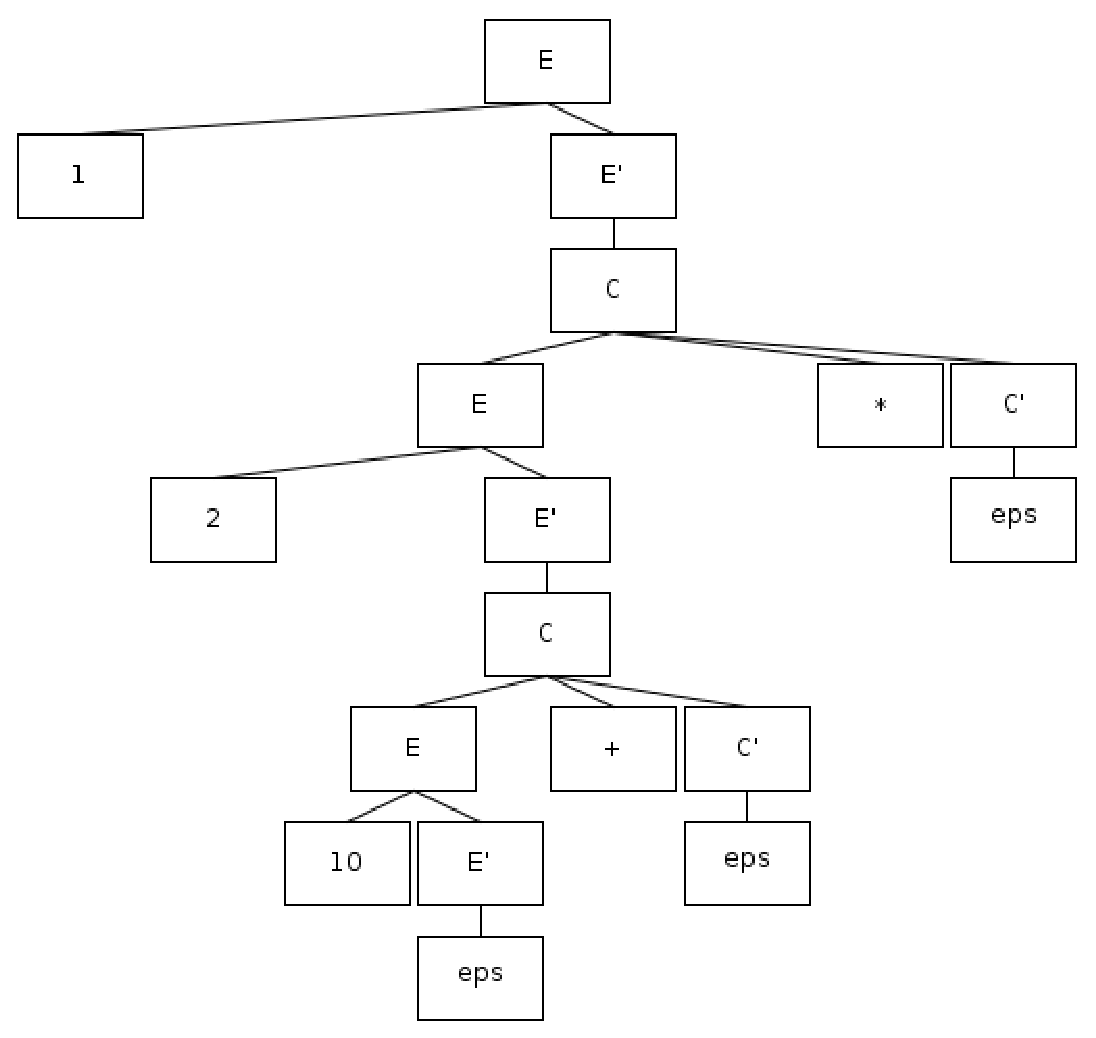
\includegraphics{test1.eps} 

\subsection{Тест 2}

\texttt{666} --- одно число

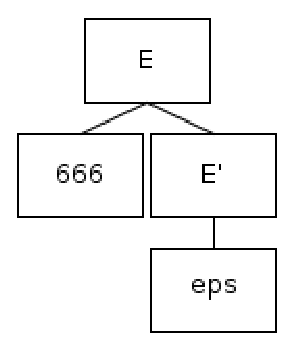
\includegraphics{test2.eps}

\subsection{Тест 3}

\texttt{7 13 -} --- простое выражение.

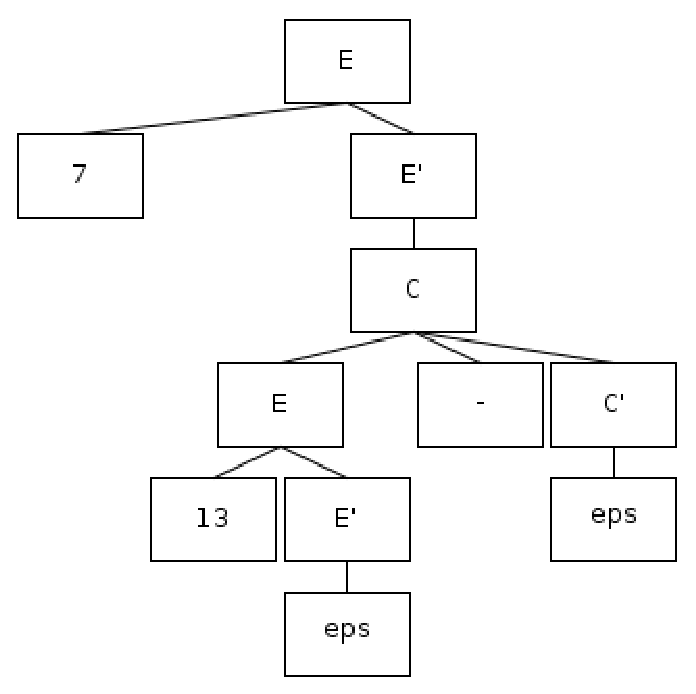
\includegraphics{test3.eps} 

\subsection{Тест 4}

\texttt{2 9 + 4 *} --- имитация скобок.

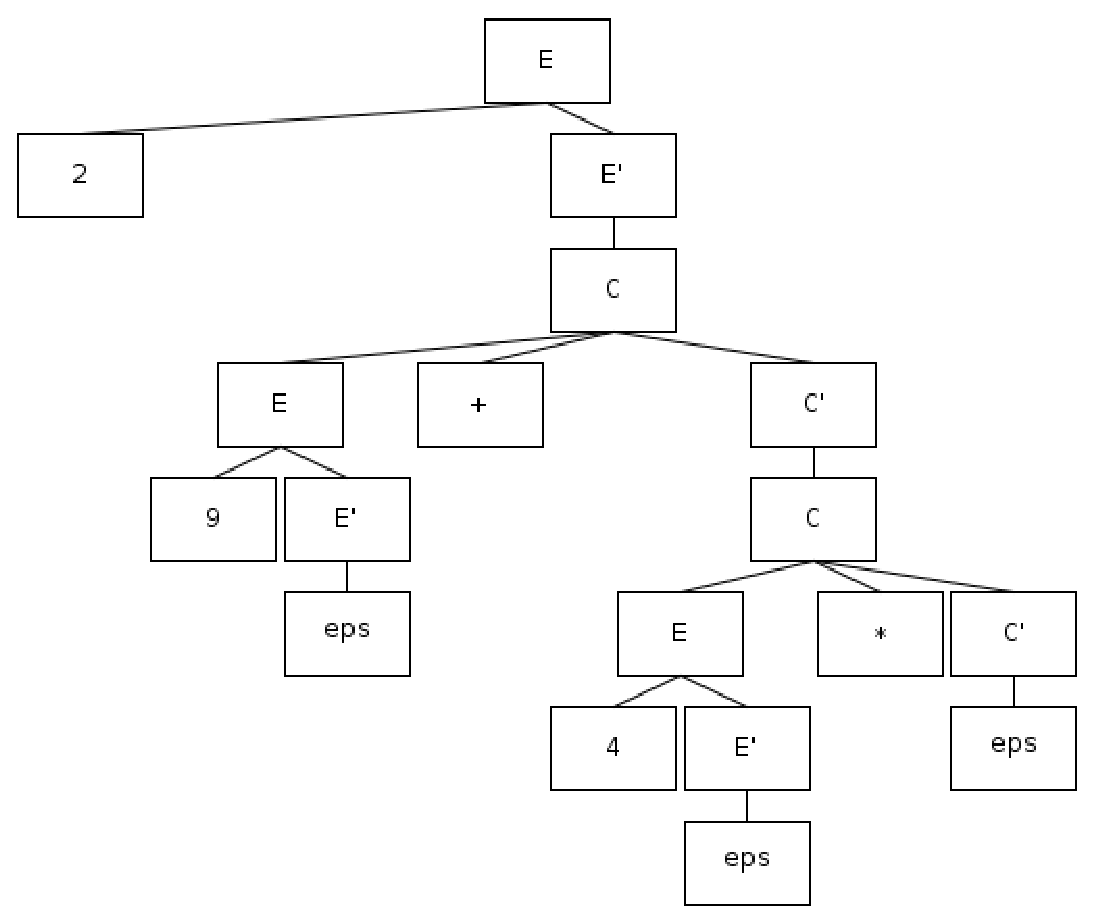
\includegraphics[width=110mm]{test4.eps} 

\subsection{Тест 5}

\texttt{4 2 - 6 0 * +} --- имитация скобок, длиннее.

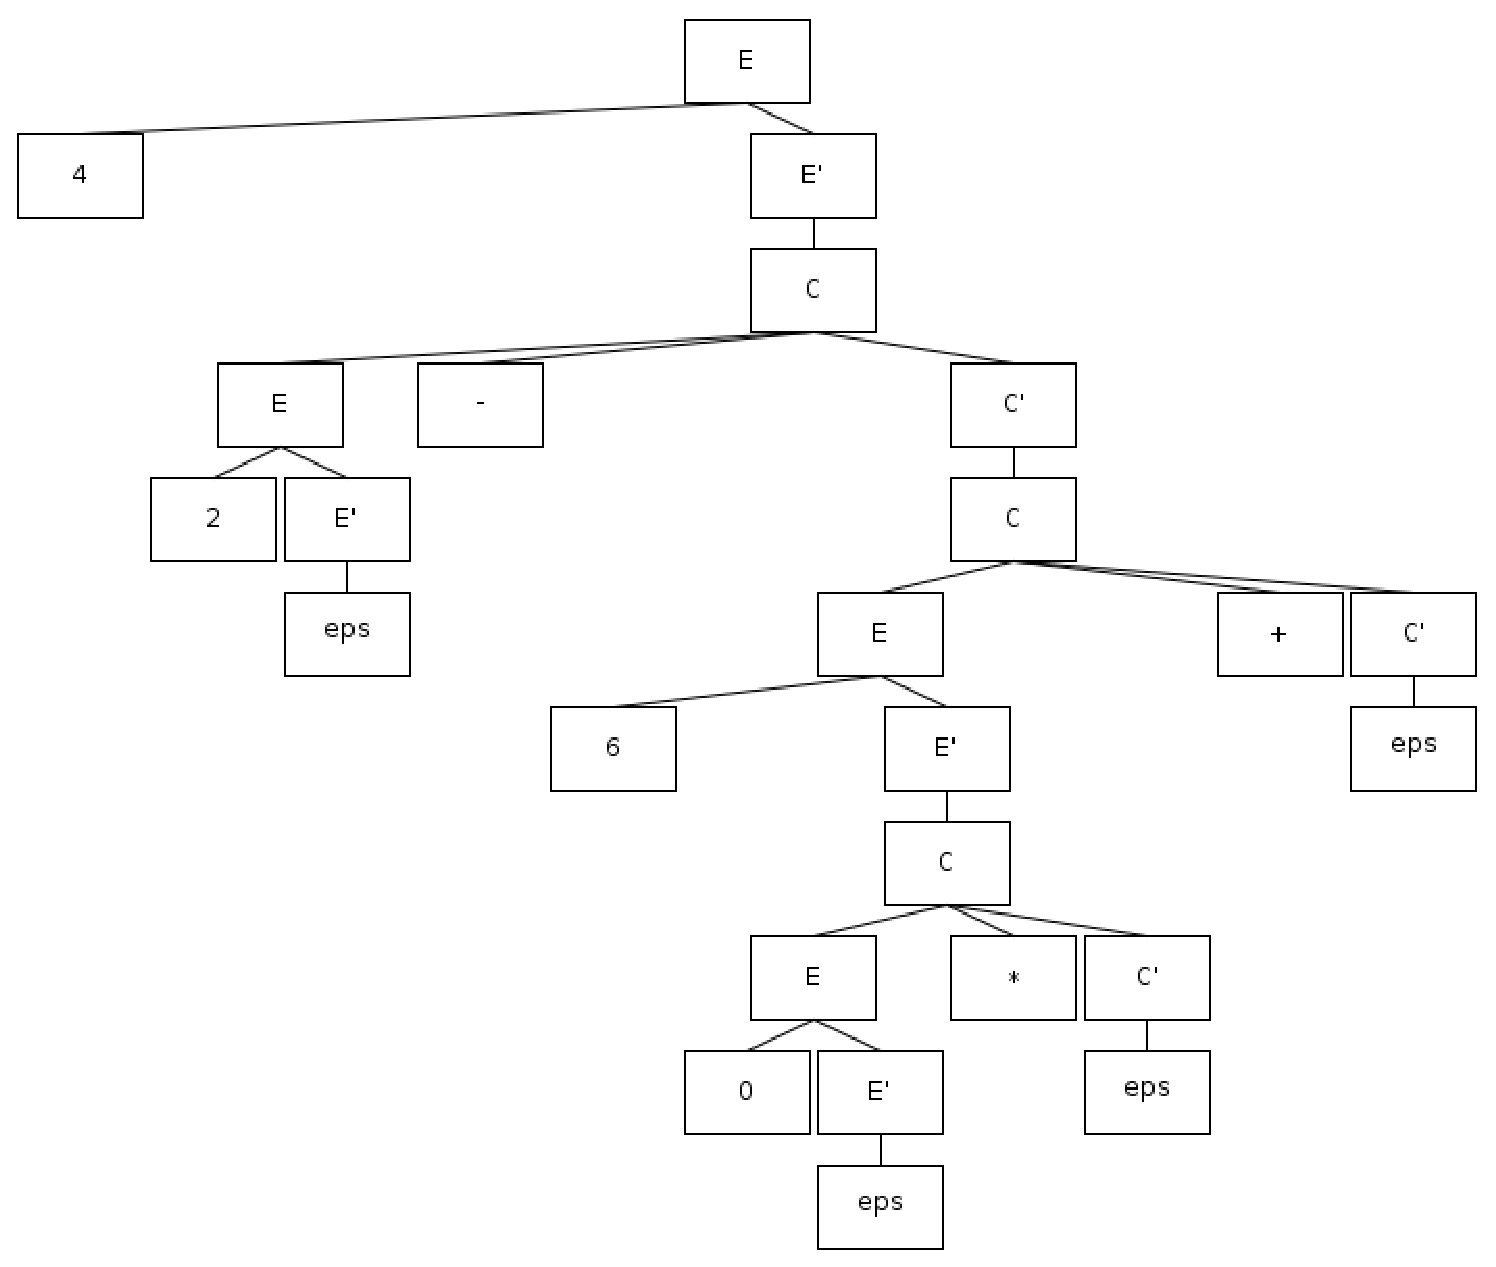
\includegraphics[width=110mm]{test5.eps} 

\subsection{Тест 6}

\texttt{1 2 * 3 4 5 - * * 6 +} --- длинное выражение.

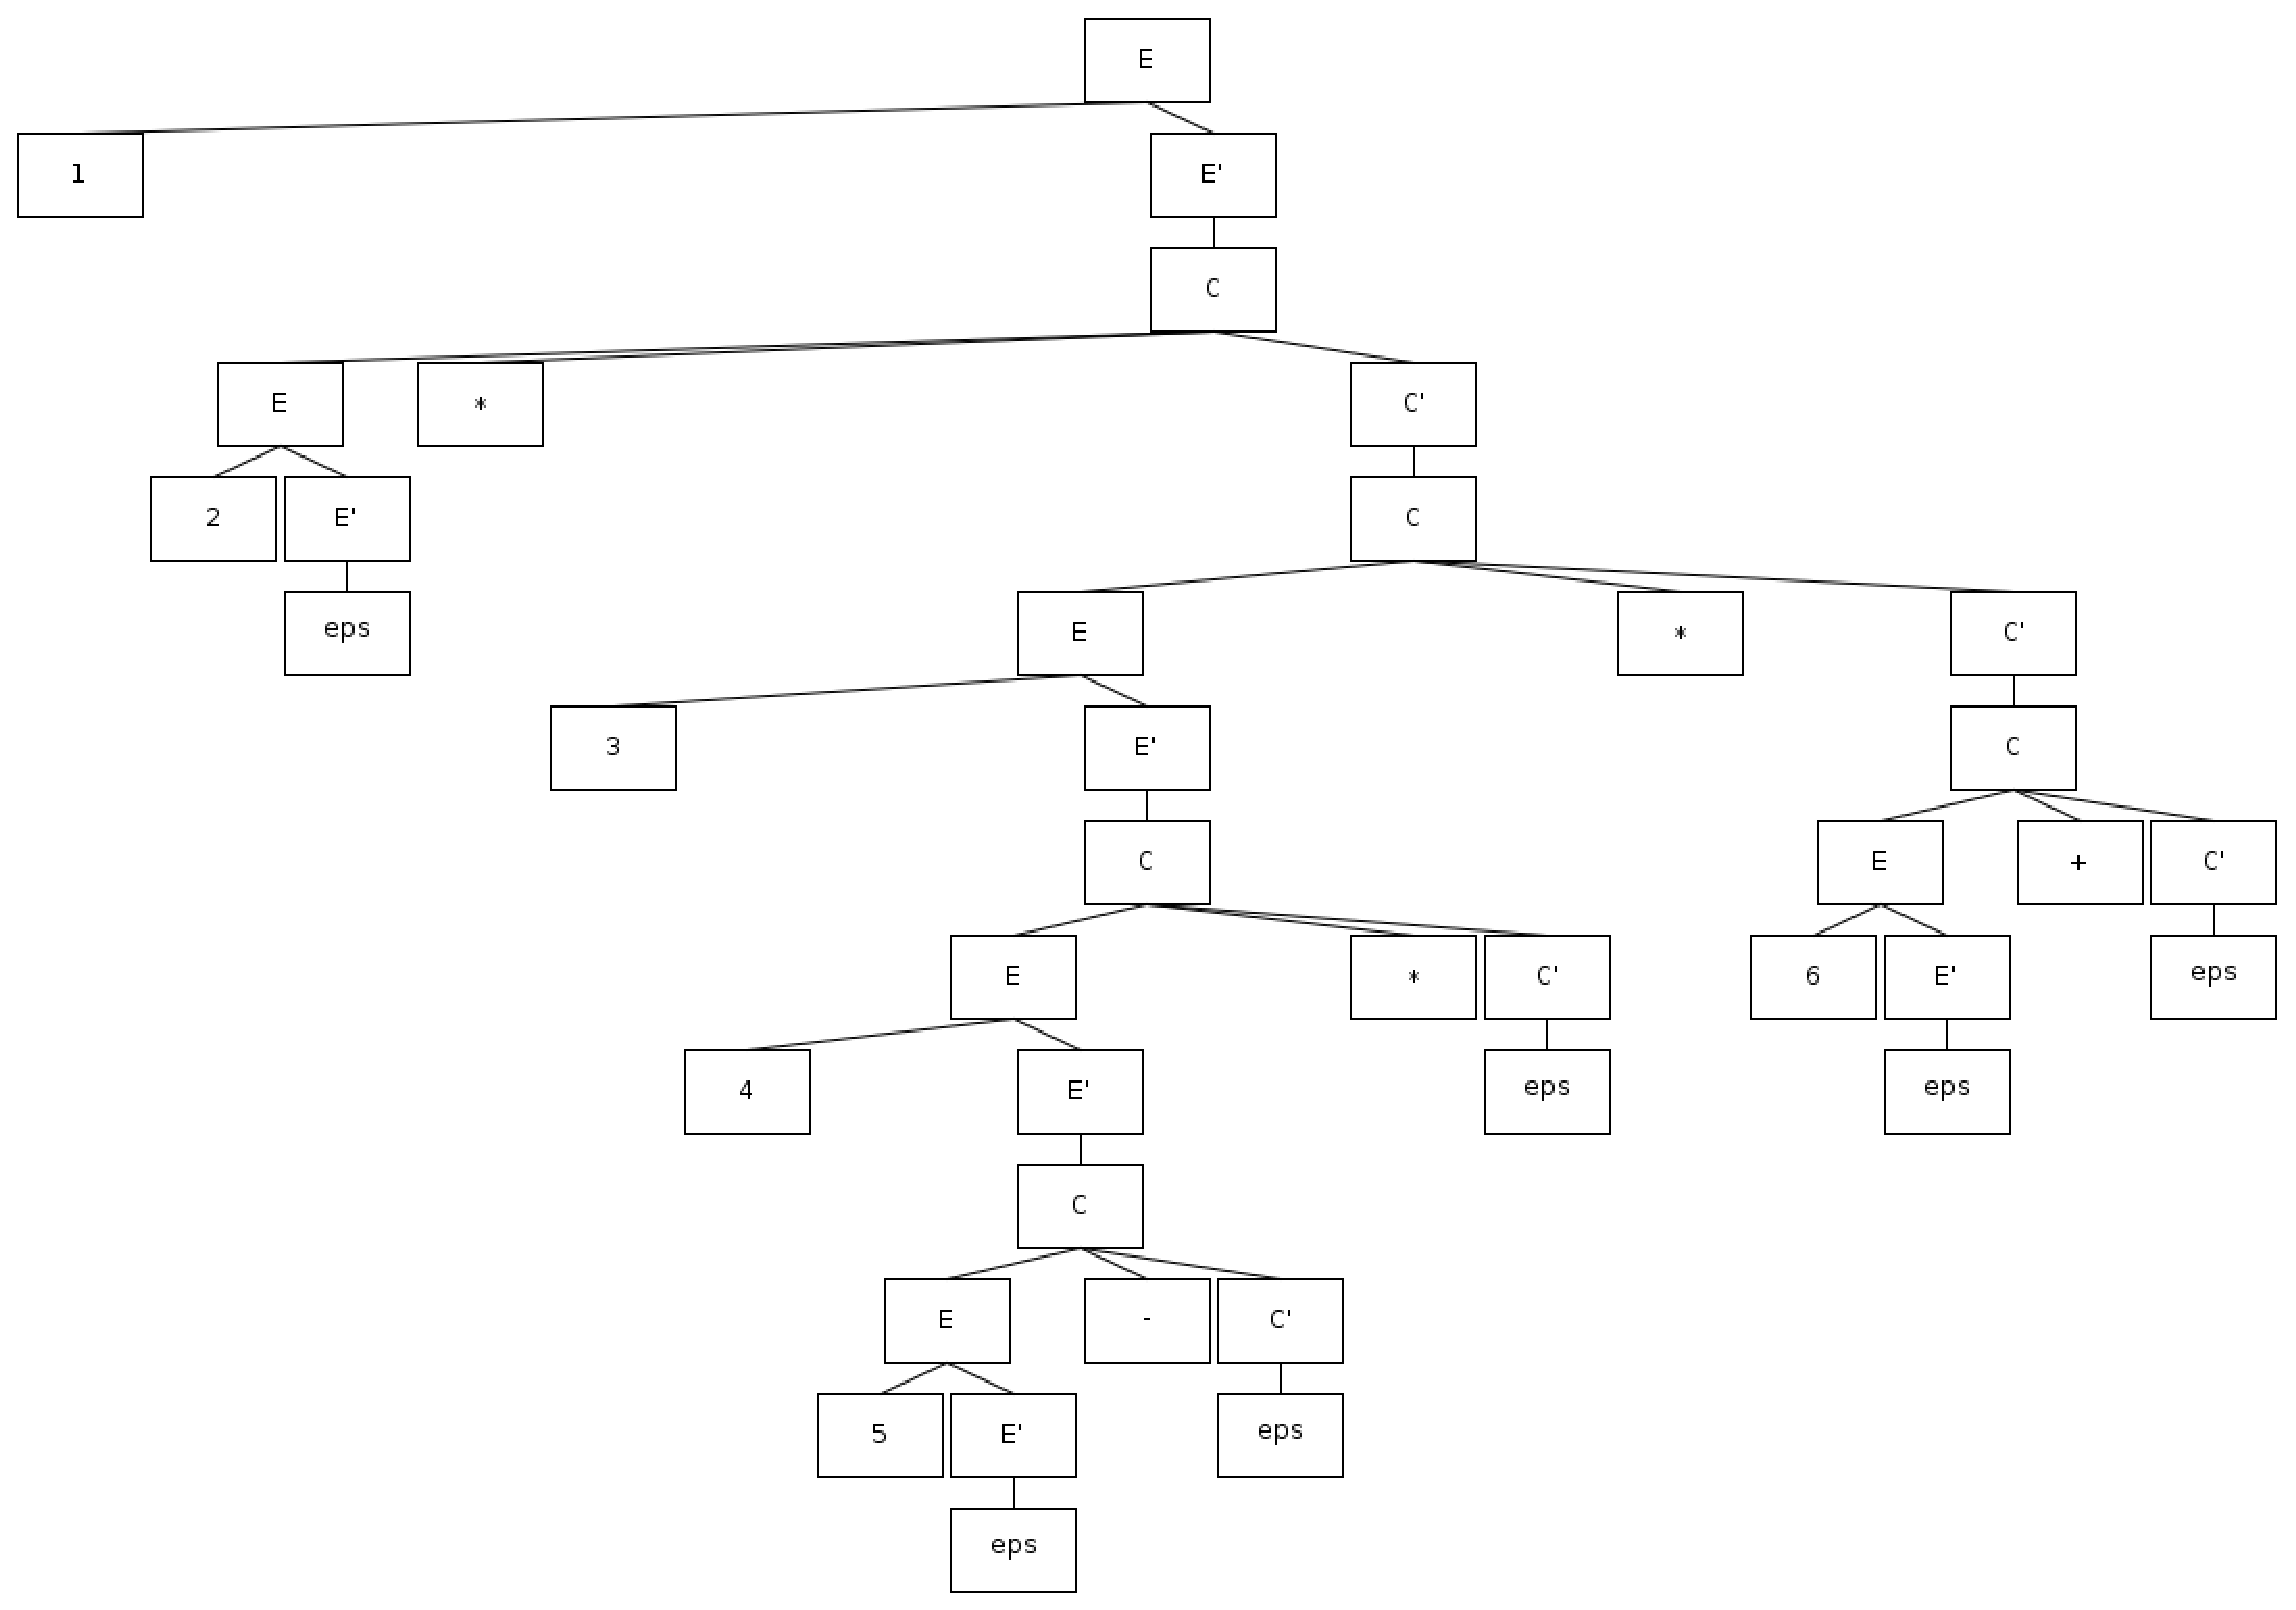
\includegraphics[width=130mm]{test6.eps} 

\subsection{Тест 7}

\texttt{4 9 + *} --- лишняя операция.

Ошибка. \texttt{End of expression expected, but * found at position 6}

\subsection{Тест 8}

\texttt{-} --- нет цифр.

Ошибка. \texttt{Number expected at position 1}

\subsection{Тест 9}

\texttt{11 22 33 +} --- не хватает операции.

Ошибка. \texttt{Operation sign expected at position 10}

\subsection{Тест 10}

\texttt{7 3 - 5} --- не хватает операции.

Ошибка. \texttt{Operation sign expected at position 7}

\subsection{Тест 11}

\texttt{1 2 -*} --- лишняя операция.

Ошибка. \texttt{End of expression expected, but * found at position 5}

\subsection{Тест 12}

\texttt{bad + test} --- некорректное выражение.

Ошибка. \texttt{character b at position 0}.